\chapter{Teoría de juegos}

En este capítulo nos centraremos en juegos de dos jugadores que no
contienen elementos aleatorios. Nuestro objetivo es encontrar una
estrategia que podamos seguir para ganar el juego sin importar lo
que haga el rival, si tal estrategia existe.

Resulta que hay una estrategia general para este tipo de juegos,
y podemos analizarlas utilizando la \key{teoría del nim}. Primero,
analizaremos juegos simples donde los jugadores quitan palos de
unas pilas, y luego de esto generalizaremos la estrategia usada
a otros juegos.

\section{Estados de juego}

Consideremos un juego donde inicialmente hay una pila de $n$ palos.
Los jugadores $A$ y $B$ se mueven en turnos. En cada turno, el jugador
debe quitar 1, 2, o 3 palos de la pila, y el jugador que quite el
último palo gana el juego.

Por ejemplo, si $n=10$, el juego puede proceder de la siguiente manera:
\begin{itemize}[noitemsep]
    \item Jugador $A$ quita 2 palos (quedan 8 palos).
    \item Jugador $B$ quita 3 palos (quedan 5 palos).
    \item Jugador $A$ quita 1 palo (quedan 4 palos).
    \item Jugador $B$ quita 2 palos (quedan 2 palos).
    \item Jugador $A$ quita 2 palos y gana.
\end{itemize}

Este juego consiste de los estados $0,1,2,\ldots,n$, donde el número
del estado corresponde al número de palos restantes.

\subsubsection{Estados ganadores y perdedores}

\index{estado ganador}
\index{estado perdedor}

Un \key{estado ganador} es un estado donde el jugador ganará el juego si
juega óptimamente, y un \key{estado perdedor} es aquel donde el jugador
perderá el juego si su rival juega óptimamente. Resulta que podemos
clasificar todos los estados de un juego como ganadores o perdedores.

En el juego anterior, el estado 0 es claramente un estado perdedor, porque
el jugador no puede realizar ningún movimiento y el rival ya ganó. Los
estados 1, 2, y 3 son estados ganadores, porque podemos quitar 1, 2, o 3
palos y ganar el juego.

El estado 4, por su parte, es un estado perdedor, porque cualquier
movimiento resulta en un estado ganador para el rival.

Más generalmente, si hay un movimiento que nos lleva del estado actual
a un estado perdedor (para el rival), el estado actual es ganador,
y de lo contrario es perdedor. Usando esta observación,
podemos clasificar todos los estados de un juego, comenzando con los
estados perdedores sin movimientos posibles.

Los estados $0 \ldots 15$ del anterior juego pueden clasificarse de la
siguiente manera ($G$ denota un estado ganador y $P$ un estado perdedor):
\begin{center}
    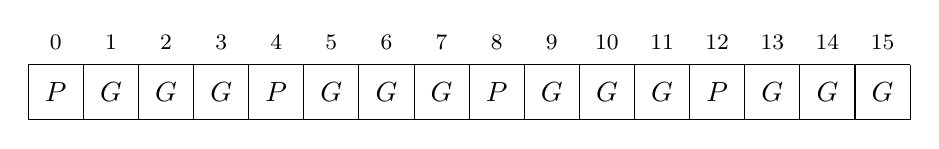
\begin{tikzpicture}[scale=0.7]
        \draw (0,0) grid (16,1);

        \node at (0.5,0.5) {$P$};
        \node at (1.5,0.5) {$G$};
        \node at (2.5,0.5) {$G$};
        \node at (3.5,0.5) {$G$};
        \node at (4.5,0.5) {$P$};
        \node at (5.5,0.5) {$G$};
        \node at (6.5,0.5) {$G$};
        \node at (7.5,0.5) {$G$};
        \node at (8.5,0.5) {$P$};
        \node at (9.5,0.5) {$G$};
        \node at (10.5,0.5) {$G$};
        \node at (11.5,0.5) {$G$};
        \node at (12.5,0.5) {$P$};
        \node at (13.5,0.5) {$G$};
        \node at (14.5,0.5) {$G$};
        \node at (15.5,0.5) {$G$};

        \footnotesize
        \node at (0.5,1.4) {$0$};
        \node at (1.5,1.4) {$1$};
        \node at (2.5,1.4) {$2$};
        \node at (3.5,1.4) {$3$};
        \node at (4.5,1.4) {$4$};
        \node at (5.5,1.4) {$5$};
        \node at (6.5,1.4) {$6$};
        \node at (7.5,1.4) {$7$};
        \node at (8.5,1.4) {$8$};
        \node at (9.5,1.4) {$9$};
        \node at (10.5,1.4) {$10$};
        \node at (11.5,1.4) {$11$};
        \node at (12.5,1.4) {$12$};
        \node at (13.5,1.4) {$13$};
        \node at (14.5,1.4) {$14$};
        \node at (15.5,1.4) {$15$};
    \end{tikzpicture}
\end{center}

Es fácil analizar este juego: un estado $k$ es perdedor si $k$ es divisible
por 4, y de lo contrario es un estado ganador. Una manera óptima de jugar
el juego es siempre elegir el movimiento tras el cual el número de palos
sea divisible por 4. Finalmente, no quedan palos y el rival ha perdido.

Por supuesto, esta estrategia requiere que el número de palos \emph{no} sea
divisible por 4 cuando toca nuestro turno. Si lo es, no hay nada que podamos
hacer y el rival ganará si juega óptimamente.

\subsubsection{Grafo de estados}

Ahora consideremos otro juego de palos, en el cual cada estado $k$ nos
permite quitar cualquier número $x$ de palos tal que $x$ sea menor que $k$
y un divisor de $k$. Por ejemplo, en el estado 8 podemos quitar 1, 2, o 4
palos, pero en el estado 7 solo podemos quitar 1 palo.

La siguiente imagen demuestra los estados $1 \ldots 9$ del juego en un
\key{grafo de estados}, cuyos nodos son los estados y aristas son los
movimientos entre ellos.

\begin{center}
    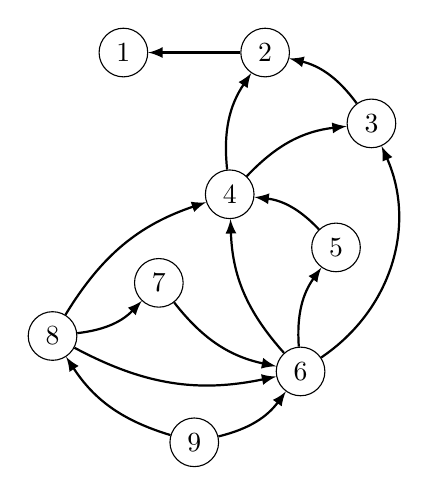
\begin{tikzpicture}[scale=0.9]
        \node[draw, circle] (1) at (0,0) {$1$};
        \node[draw, circle] (2) at (2,0) {$2$};
        \node[draw, circle] (3) at (3.5,-1) {$3$};
        \node[draw, circle] (4) at (1.5,-2) {$4$};
        \node[draw, circle] (5) at (3,-2.75) {$5$};
        \node[draw, circle] (6) at (2.5,-4.5) {$6$};
        \node[draw, circle] (7) at (0.5,-3.25) {$7$};
        \node[draw, circle] (8) at (-1,-4) {$8$};
        \node[draw, circle] (9) at (1,-5.5) {$9$};

        \path[draw,thick,->,>=latex] (2) -- (1);
        \path[draw,thick,->,>=latex] (3) edge [bend right=20] (2);
        \path[draw,thick,->,>=latex] (4) edge [bend left=20] (2);
        \path[draw,thick,->,>=latex] (4) edge [bend left=20] (3);
        \path[draw,thick,->,>=latex] (5) edge [bend right=20] (4);
        \path[draw,thick,->,>=latex] (6) edge [bend left=20] (5);
        \path[draw,thick,->,>=latex] (6) edge [bend left=20] (4);
        \path[draw,thick,->,>=latex] (6) edge [bend right=40] (3);
        \path[draw,thick,->,>=latex] (7) edge [bend right=20] (6);
        \path[draw,thick,->,>=latex] (8) edge [bend right=20] (7);
        \path[draw,thick,->,>=latex] (8) edge [bend right=20] (6);
        \path[draw,thick,->,>=latex] (8) edge [bend left=20] (4);
        \path[draw,thick,->,>=latex] (9) edge [bend left=20] (8);
        \path[draw,thick,->,>=latex] (9) edge [bend right=20] (6);
    \end{tikzpicture}
\end{center}

El estado final en este juego siempre es 1, un estado perdedor,
porque no existen movimientos válidos. La clasificación de los estados
$1 \ldots 9$ es la siguiente:

\begin{center}
    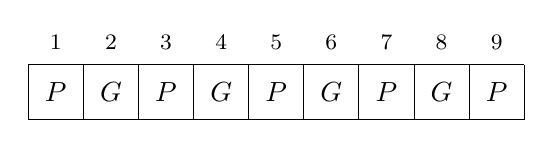
\begin{tikzpicture}[scale=0.7]
        \draw (1,0) grid (10,1);

        \node at (1.5,0.5) {$P$};
        \node at (2.5,0.5) {$G$};
        \node at (3.5,0.5) {$P$};
        \node at (4.5,0.5) {$G$};
        \node at (5.5,0.5) {$P$};
        \node at (6.5,0.5) {$G$};
        \node at (7.5,0.5) {$P$};
        \node at (8.5,0.5) {$G$};
        \node at (9.5,0.5) {$P$};

        \footnotesize
        \node at (1.5,1.4) {$1$};
        \node at (2.5,1.4) {$2$};
        \node at (3.5,1.4) {$3$};
        \node at (4.5,1.4) {$4$};
        \node at (5.5,1.4) {$5$};
        \node at (6.5,1.4) {$6$};
        \node at (7.5,1.4) {$7$};
        \node at (8.5,1.4) {$8$};
        \node at (9.5,1.4) {$9$};
    \end{tikzpicture}
\end{center}

Sorprendentemente, en este juego, todos los estados de número par son
ganadores, y todos los estados de número impar son perdedores.

\section{El juego del nim}

\index{juego del nim}

El \key{juego del nim} es un juego simple con un importante rol en la
teoría de juegos, ya que muchos otros juegos pueden jugarse usando la misma
estrategia. Primero nos centraremos en nim y luego generalizaremos su
estrategia a otros juegos.

Hay $n$ pilas en el juego del nim, y cada pila contiene algún número de
palos. Los jugadores se mueven en turnos, y en cada turno, el jugador
elige una pila que todavía contenga palos y quita cualquier número de palos
de ella. El ganador es el jugador que quite el último palo.

Los estados en el nim tienen la forma $[x_1,x_2,\ldots,x_n]$, donde $x_k$
denota el número de palos en la pila $k$. Por ejemplo, $[10,12,5]$ es un
juego donde hay tres pilas con 10, 12, y 5 palos. El estado $[0,0,\ldots,0]$
es un estado perdedor, porque no es posible quitar ningún palo, y este
siempre es el estado final.

\subsubsection{Análisis}
\index{suma nim}

Resulta que podemos fácilmente clasificar cualquier estado del nim si
calculamos la \key{suma nim} $s = x_1 \oplus x_2 \oplus \cdots \oplus x_n$,
donde $\oplus$ es la operación xor.\footnote{La estrategia óptima para el
    nim fue publicada en 1901 por C. L. Bouton \cite{bou01}.}
Los estados cuyas sumas nim sean 0 son perdedores, y el resto son ganadores.
Por ejemplo, la suma nim de $[10,12,5]$ es $10 \oplus 12 \oplus 5 = 3$,
por lo que el estado es ganador.

¿Pero cómo están relacionados la suma nim y el juego del nim? Podemos
explicar esto viendo cómo la suma nim cambia cuando el estado de juego
cambia.

\textit{Estados perdedores}: El estado final $[0,0,\ldots,0]$ es un
estado perdedor, y su suma nim es 0, como era de esperar. En los otros
juegos perdedores, cualquier movimiento resulta en un estado ganador,
porque cuando un solo valor $x_k$ cambia, la suma nim también cambia,
así que es diferente de 0 después del movimiento.

\textit{Estados ganadores}: Podemos mover a un estado perdedor si existe
cualquier pila $k$ para la cual $x_k \oplus s < x_k$. En este caso, podemos
quitar palos de la pila $k$ tal que contenga $x_k \oplus s$ palos, que
llevará a un estado perdedor. Siempre existe tal pila, donde $x_k$ tiene
un bit uno en la posición del bit uno más a la izquierda de $s$.

Por ejemplo, considera el estado $[10,12,5]$. El estado es ganador, porque
su suma nim es 3. Por ende, tiene que haber un movimiento que lleve a
un estado perdedor. Ahora encontraremos un movimiento tal.

La suma nim del estado es la siguiente:

\begin{center}
    \begin{tabular}{r|r}
        10 & \texttt{1010} \\
        12 & \texttt{1100} \\
        5  & \texttt{0101} \\
        \hline
        3  & \texttt{0011} \\
    \end{tabular}
\end{center}

En este caso, la pila con 10 palos es la única pila que tiene un bit uno
en la posición del bit uno más a la izquierda de la suma nim:

\begin{center}
    \begin{tabular}{r|r}
        10 & \texttt{10\underline{1}0} \\
        12 & \texttt{1100}             \\
        5  & \texttt{0101}             \\
        \hline
        3  & \texttt{00\underline{1}1} \\
    \end{tabular}
\end{center}

El nuevo tamaño de la pila debe ser $10 \oplus 3 = 9$, así que quitaremos
solo un palo. Luego de esto, el estado será $[9,12,5]$, un estado perdedor:

\begin{center}
    \begin{tabular}{r|r}
        9  & \texttt{1001} \\
        12 & \texttt{1100} \\
        5  & \texttt{0101} \\
        \hline
        0  & \texttt{0000} \\
    \end{tabular}
\end{center}

\subsubsection{Juego misère}

\index{juego misère}

En un \key{juego misère}, el objetivo del juego es el opuesto, así que
el jugador que quita el último palo pierde el juego. Resulta que la versión
misère del nim puede jugarse óptimamente casi como el juego del nim normal.

La idea es primero jugar el juego misère como el juego normal, pero cambiar
la estrategia al final del juego. La nueva estrategia se introducirá
en una situación donde cada pila contendrá como mucho un palo luego del
siguiente movimiento.

En el juego normal, deberíamos elegir un movimiento después del cual
exista un número par de pilas con un palo. Sin embargo, en el juego
misère, elegimos un movimiento tal que quede un número impar de pilas
con un palo.

Esta estrategia funciona porque en un estado donde la estrategia cambia
siempre aparece en el juego, y este estado es un estado ganador, porque
contiene exactamente una pila con más de un palo por lo que la suma nim
es 0.

\section{Teorema de Sprague--Grundy}

\index{teorema de!Sprague--Grundy}

El \key{teorema de Sprague--Grundy}\footnote{Este teorema fue descubierto
    independientemente por R. Sprague \cite{spr35} y P. M. Grundy \cite{gru39}.}
generaliza la estrategia utilizada en el juego del nim a todos los juegos
que cumplan los siguientes requerimientos:

\begin{itemize}[noitemsep]
    \item Hay dos jugadores que se mueven en turnos.
    \item El juego consiste de estados, y los movimientos posibles en
          un estado no dependen del jugador actual.
    \item El juego termina cuando ya no se puede hacer un movimiento.
    \item El juego definitivamente termina tarde o temprano.
    \item Los jugadores tienen información completa sobre los estados
          y movimientos permitidos, y no existe la aleatoriedad.
\end{itemize}

La idea es calcular, para cada estado de juego, un número de Grundy
que corresponde al número de palos en una pila del nim. Una vez que
sabemos los números de Grundy de todos los estados, podemos jugar el
juego como un juego del nim.

\subsubsection{Números de Grundy}

\index{número de Grundy}
\indexalt{nimber}
\index{mex (función)}

El \key{número de Grundy} de un estado de juego es
\[\mex(\{g_1,g_2,\ldots,g_n\}),\] donde $g_1,g_2,\ldots,g_n$ son
los números de Grundy de los estados a cuales nos podemos mover,
y la función mex devuelve el mínimo número no negativo que no se
encuentre en el conjunto dado. Por ejemplo, $\mex(\{0,1,3\})=2$.
Si no hay movimientos posibles en un estado, su número de Grundy
es 0, porque $\mex(\emptyset)=0$.

Por ejemplo, en el grafo de estados
\begin{center}
    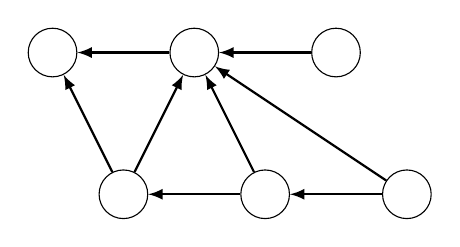
\begin{tikzpicture}[scale=0.9]
        \node[draw, circle] (1) at (0,0) {\phantom{0}};
        \node[draw, circle] (2) at (2,0) {\phantom{0}};
        \node[draw, circle] (3) at (4,0) {\phantom{0}};
        \node[draw, circle] (4) at (1,-2) {\phantom{0}};
        \node[draw, circle] (5) at (3,-2) {\phantom{0}};
        \node[draw, circle] (6) at (5,-2) {\phantom{0}};

        \path[draw,thick,->,>=latex] (2) -- (1);
        \path[draw,thick,->,>=latex] (3) -- (2);
        \path[draw,thick,->,>=latex] (5) -- (4);
        \path[draw,thick,->,>=latex] (6) -- (5);
        \path[draw,thick,->,>=latex] (4) -- (1);
        \path[draw,thick,->,>=latex] (4) -- (2);
        \path[draw,thick,->,>=latex] (5) -- (2);
        \path[draw,thick,->,>=latex] (6) -- (2);
    \end{tikzpicture}
\end{center}
los números de Grundy son los siguientes:
\begin{center}
    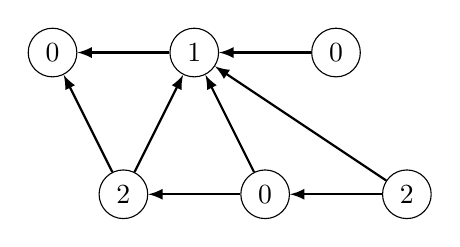
\begin{tikzpicture}[scale=0.9]
        \node[draw, circle] (1) at (0,0) {0};
        \node[draw, circle] (2) at (2,0) {1};
        \node[draw, circle] (3) at (4,0) {0};
        \node[draw, circle] (4) at (1,-2) {2};
        \node[draw, circle] (5) at (3,-2) {0};
        \node[draw, circle] (6) at (5,-2) {2};

        \path[draw,thick,->,>=latex] (2) -- (1);
        \path[draw,thick,->,>=latex] (3) -- (2);
        \path[draw,thick,->,>=latex] (5) -- (4);
        \path[draw,thick,->,>=latex] (6) -- (5);
        \path[draw,thick,->,>=latex] (4) -- (1);
        \path[draw,thick,->,>=latex] (4) -- (2);
        \path[draw,thick,->,>=latex] (5) -- (2);
        \path[draw,thick,->,>=latex] (6) -- (2);
    \end{tikzpicture}
\end{center}
El número de Grundy de un estado perdedor es 0, y el número de Grundy
de un estado ganador es un número positivo.

El número de Grundy de un estado corresponde al número de palos en una
pila del nim. Si el número de Grundy es 0, solamente podemos movernos a
aquellos estados cuyo número de Grundy sea positivo, y si el número es
positivo, podemos movernos a aquellos estados cuyo número de Grundy sea
menor.

Por ejemplo, considera un juego donde los jugadores mueven una figura en un
laberinto. Cada cuadrado del laberinto es un piso o una pared. En cada turno,
el jugador debe mover la figura un número de pasos hacia arriba o a la
izquierda. El ganador del juego es aquel jugador que haga el último
movimiento.

La siguiente imagen muestra un posible estado inicial del juego, donde
@ denota a la figura y $\times$ denota cuadrados a los que puede moverse.

\begin{center}
    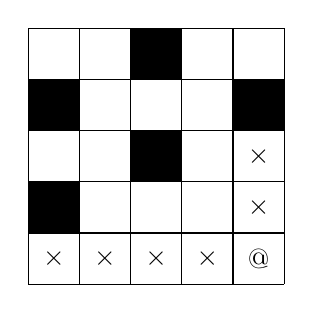
\begin{tikzpicture}[scale=.65]
        \begin{scope}
            \fill [color=black] (0, 1) rectangle (1, 2);
            \fill [color=black] (0, 3) rectangle (1, 4);
            \fill [color=black] (2, 2) rectangle (3, 3);
            \fill [color=black] (2, 4) rectangle (3, 5);
            \fill [color=black] (4, 3) rectangle (5, 4);

            \draw (0, 0) grid (5, 5);

            \node at (4.5,0.5) {@};
            \node at (3.5,0.5) {$\times$};
            \node at (2.5,0.5) {$\times$};
            \node at (1.5,0.5) {$\times$};
            \node at (0.5,0.5) {$\times$};
            \node at (4.5,1.5) {$\times$};
            \node at (4.5,2.5) {$\times$};

        \end{scope}
    \end{tikzpicture}
\end{center}

Los estados del juego son todos cuadrados tipo piso en el laberinto. En el
laberinto de arriba, los números de Grundy son los siguientes:

\begin{center}
    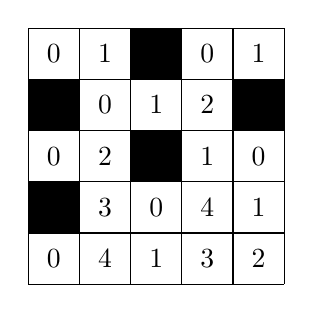
\begin{tikzpicture}[scale=.65]
        \begin{scope}
            \fill [color=black] (0, 1) rectangle (1, 2);
            \fill [color=black] (0, 3) rectangle (1, 4);
            \fill [color=black] (2, 2) rectangle (3, 3);
            \fill [color=black] (2, 4) rectangle (3, 5);
            \fill [color=black] (4, 3) rectangle (5, 4);

            \draw (0, 0) grid (5, 5);

            \node at (0.5,4.5) {0};
            \node at (1.5,4.5) {1};
            \node at (2.5,4.5) {};
            \node at (3.5,4.5) {0};
            \node at (4.5,4.5) {1};

            \node at (0.5,3.5) {};
            \node at (1.5,3.5) {0};
            \node at (2.5,3.5) {1};
            \node at (3.5,3.5) {2};
            \node at (4.5,3.5) {};

            \node at (0.5,2.5) {0};
            \node at (1.5,2.5) {2};
            \node at (2.5,2.5) {};
            \node at (3.5,2.5) {1};
            \node at (4.5,2.5) {0};

            \node at (0.5,1.5) {};
            \node at (1.5,1.5) {3};
            \node at (2.5,1.5) {0};
            \node at (3.5,1.5) {4};
            \node at (4.5,1.5) {1};

            \node at (0.5,0.5) {0};
            \node at (1.5,0.5) {4};
            \node at (2.5,0.5) {1};
            \node at (3.5,0.5) {3};
            \node at (4.5,0.5) {2};
        \end{scope}
    \end{tikzpicture}
\end{center}

Por ende, cada estado del juego del laberinto corresponde a una pila en
el juego del nim. Por ejemplo, el número de Grundy para el cuadrado
inferior derecho es 2, así que es un estado ganador. Podemos alcanzar un
estado perdedor y ganar el juego si nos movemos cuatro pasos a la izquierda
o dos pasos hacia arriba.

Ten en cuenta que a diferencia del nim original, puede ser posible
movernos a un estado cuyo número de Grundy sea superior que el número
Grundy del estado actual. Sin embargo, el rival siempre puede elegir un
movimiento que cancele el nuestro, así que no es posible escapar de un
estado perdedor.

\subsubsection{Subjuegos}

Ahora digamos que nuestro juego consiste de subjuegos, y en cada turno,
el jugador primero elige un subjuego y luego un movimiento en el subjuego.
El juego termina cuando no es posible hacer algún movimiento en algún
subjuego.

En este caso, el número de Grundy de un juego es la suma nim de los números
Grundy de sus subjuegos. El juego puede jugarse como un nim si
calculamos todos los números de Grundy para los subjuegos y luego su suma nim.

Por ejemplo, considera un juego que consiste de tres laberintos. En este
juego, en cada turno, el jugador elige uno de los laberintos y mueve
la figura. Asume que el estado inicial del juego es el siguiente:

\begin{center}
    \begin{tabular}{ccc}
        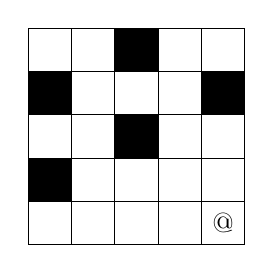
\begin{tikzpicture}[scale=.55]
            \begin{scope}
                \fill [color=black] (0, 1) rectangle (1, 2);
                \fill [color=black] (0, 3) rectangle (1, 4);
                \fill [color=black] (2, 2) rectangle (3, 3);
                \fill [color=black] (2, 4) rectangle (3, 5);
                \fill [color=black] (4, 3) rectangle (5, 4);

                \draw (0, 0) grid (5, 5);

                \node at (4.5,0.5) {@};

            \end{scope}
        \end{tikzpicture}
         &
        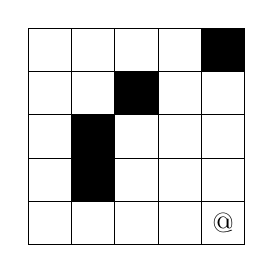
\begin{tikzpicture}[scale=.55]
            \begin{scope}
                \fill [color=black] (1, 1) rectangle (2, 3);
                \fill [color=black] (2, 3) rectangle (3, 4);
                \fill [color=black] (4, 4) rectangle (5, 5);

                \draw (0, 0) grid (5, 5);

                \node at (4.5,0.5) {@};

            \end{scope}
        \end{tikzpicture}
         &
        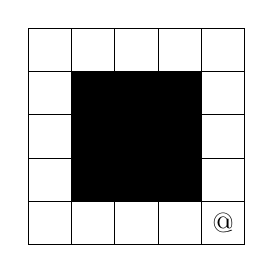
\begin{tikzpicture}[scale=.55]
            \begin{scope}
                \fill [color=black] (1, 1) rectangle (4, 4);

                \draw (0, 0) grid (5, 5);

                \node at (4.5,0.5) {@};
            \end{scope}
        \end{tikzpicture}
    \end{tabular}
\end{center}

Los números de Grundy para los laberintos son:

\begin{center}
    \begin{tabular}{ccc}
        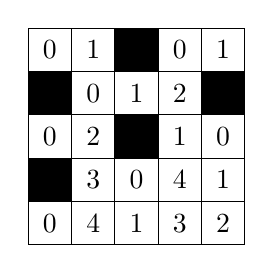
\begin{tikzpicture}[scale=.55]
            \begin{scope}
                \fill [color=black] (0, 1) rectangle (1, 2);
                \fill [color=black] (0, 3) rectangle (1, 4);
                \fill [color=black] (2, 2) rectangle (3, 3);
                \fill [color=black] (2, 4) rectangle (3, 5);
                \fill [color=black] (4, 3) rectangle (5, 4);

                \draw (0, 0) grid (5, 5);

                \node at (0.5,4.5) {0};
                \node at (1.5,4.5) {1};
                \node at (2.5,4.5) {};
                \node at (3.5,4.5) {0};
                \node at (4.5,4.5) {1};

                \node at (0.5,3.5) {};
                \node at (1.5,3.5) {0};
                \node at (2.5,3.5) {1};
                \node at (3.5,3.5) {2};
                \node at (4.5,3.5) {};

                \node at (0.5,2.5) {0};
                \node at (1.5,2.5) {2};
                \node at (2.5,2.5) {};
                \node at (3.5,2.5) {1};
                \node at (4.5,2.5) {0};

                \node at (0.5,1.5) {};
                \node at (1.5,1.5) {3};
                \node at (2.5,1.5) {0};
                \node at (3.5,1.5) {4};
                \node at (4.5,1.5) {1};

                \node at (0.5,0.5) {0};
                \node at (1.5,0.5) {4};
                \node at (2.5,0.5) {1};
                \node at (3.5,0.5) {3};
                \node at (4.5,0.5) {2};
            \end{scope}
        \end{tikzpicture}
         &
        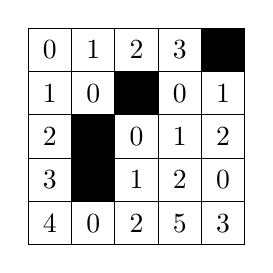
\begin{tikzpicture}[scale=.55]
            \begin{scope}
                \fill [color=black] (1, 1) rectangle (2, 3);
                \fill [color=black] (2, 3) rectangle (3, 4);
                \fill [color=black] (4, 4) rectangle (5, 5);

                \draw (0, 0) grid (5, 5);

                \node at (0.5,4.5) {0};
                \node at (1.5,4.5) {1};
                \node at (2.5,4.5) {2};
                \node at (3.5,4.5) {3};
                \node at (4.5,4.5) {};

                \node at (0.5,3.5) {1};
                \node at (1.5,3.5) {0};
                \node at (2.5,3.5) {};
                \node at (3.5,3.5) {0};
                \node at (4.5,3.5) {1};

                \node at (0.5,2.5) {2};
                \node at (1.5,2.5) {};
                \node at (2.5,2.5) {0};
                \node at (3.5,2.5) {1};
                \node at (4.5,2.5) {2};

                \node at (0.5,1.5) {3};
                \node at (1.5,1.5) {};
                \node at (2.5,1.5) {1};
                \node at (3.5,1.5) {2};
                \node at (4.5,1.5) {0};

                \node at (0.5,0.5) {4};
                \node at (1.5,0.5) {0};
                \node at (2.5,0.5) {2};
                \node at (3.5,0.5) {5};
                \node at (4.5,0.5) {3};
            \end{scope}
        \end{tikzpicture}
         &
        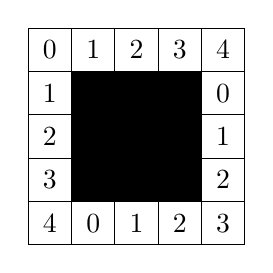
\begin{tikzpicture}[scale=.55]
            \begin{scope}
                \fill [color=black] (1, 1) rectangle (4, 4);

                \draw (0, 0) grid (5, 5);

                \node at (0.5,4.5) {0};
                \node at (1.5,4.5) {1};
                \node at (2.5,4.5) {2};
                \node at (3.5,4.5) {3};
                \node at (4.5,4.5) {4};

                \node at (0.5,3.5) {1};
                \node at (1.5,3.5) {};
                \node at (2.5,3.5) {};
                \node at (3.5,3.5) {};
                \node at (4.5,3.5) {0};

                \node at (0.5,2.5) {2};
                \node at (1.5,2.5) {};
                \node at (2.5,2.5) {};
                \node at (3.5,2.5) {};
                \node at (4.5,2.5) {1};

                \node at (0.5,1.5) {3};
                \node at (1.5,1.5) {};
                \node at (2.5,1.5) {};
                \node at (3.5,1.5) {};
                \node at (4.5,1.5) {2};

                \node at (0.5,0.5) {4};
                \node at (1.5,0.5) {0};
                \node at (2.5,0.5) {1};
                \node at (3.5,0.5) {2};
                \node at (4.5,0.5) {3};
            \end{scope}
        \end{tikzpicture}
    \end{tabular}
\end{center}

En el estado inicial, la suma nim de los números de Grundy es
$2 \oplus 3 \oplus 3 = 2$, así que el primer jugador puede ganar el juego.
Un movimiento óptimo es moverse dos pasos hacia arriba en el primer
laberinto, lo que produce la suma nim $0 \oplus 3 \oplus 3 = 0$.

\subsubsection{El juego de Grundy}

A veces un movimiento en el juego lo divide en subjuegos que son
independientes uno de otro. En este caso, el número de Grundy del juego es
\[\mex(\{g_1, g_2, \ldots, g_n \}),\] donde $n$ es el número de
movimientos posibles y
\[g_k = a_{k,1} \oplus a_{k,2} \oplus \ldots \oplus a_{k,m},\]
donde el movimiento $k$ genera subjuegos con números de Grundy
$a_{k,1},\ldots,a_{k,m}$.

\index{juego de Grundy}

Un ejemplo de tal juego es el \key{juego de Grundy}. Inicialmente, hay
una sola pila que contiene $n$ palos. En cada turno, el jugador elige
una pila y la divide en dos pilas tal que sean de distinto tamaño. El
jugador que hace el último movimiento gana el juego.

Definamos $f(n)$ como el número de Grundy de una pila que contiene $n$
palos. El número de Grundy puede calcularse recorriendo todas las maneras
de dividir la pila en dos. Por ejemplo, cuando $n=8$, las posibilidades
son $1+7$, $2+6$ y $3+5$, así que
\[f(8)=\mex(\{f(1) \oplus f(7), f(2) \oplus f(6), f(3) \oplus f(5)\}).\]

En este juego, el valor de $f(n)$ se basa en los valores de
$f(1),\ldots,f(n-1)$. Los casos base son $f(1)=f(2)=0$, porque no es
posible dividir las pilas de 1 y 2 palos. Los primeros números de Grundy son:
\[
    \begin{array}{lcl}
        f(1) & = & 0 \\
        f(2) & = & 0 \\
        f(3) & = & 1 \\
        f(4) & = & 0 \\
        f(5) & = & 2 \\
        f(6) & = & 1 \\
        f(7) & = & 0 \\
        f(8) & = & 2 \\
    \end{array}
\]
El número de Grundy para $n=8$ es 2, así que es posible ganar el juego.
El movimiento ganador es crear las pilas $1+7$, porque
$f(1) \oplus f(7) = 0$.

